\documentclass[a4paper,12pt]{article}
\usepackage{HomeWorkTemplate}
\usepackage{circuitikz}
\usepackage[shortlabels]{enumitem}
\usepackage{float}
\usepackage{hyperref}
\usepackage{tikz}
\usepackage{amsmath}
\usepackage{amssymb}
\usepackage{tcolorbox}
\usepackage{xepersian}
\settextfont{XB Niloofar}
\usetikzlibrary{arrows,automata}
\usetikzlibrary{circuits.logic.US}
\usepackage{changepage}
\newcounter{problemcounter}
\newcounter{subproblemcounter}
\setcounter{problemcounter}{1}
\setcounter{subproblemcounter}{1}
\newcommand{\problem}[1]
{
	\subsection*{
		پرسش
		\arabic{problemcounter} 
		\stepcounter{problemcounter}
		\setcounter{subproblemcounter}{1}
		#1
	}
}
\newcommand{\subproblem}{
	\textbf{\harfi{subproblemcounter})}\stepcounter{subproblemcounter}
}


\begin{document}
\handout
{آز طراحی سیستم‌های دیجیتال}
{دکتر سیاوش بیات سرمدی}
{نیم‌سال اول 1400\lr{-}1401}
{اطلاعیه}
{پرهام چاوشیان}
{98100118}
 {گزارش آزمایش دوم}
{خانم زینب رشیدی}
مطابق با دستور کار یک ماژول
$counter$
نوشته شده است که قابلیت شمارش رو به بالا و رو به پایین را دارد. زمانی که شمارنده آن برابر 0 باشد، دیگر رو به پایین شمارش نخواهد کرد. سپس یک ماژول $room$ داریم که درواقع همان کنترل‌کننده اتاق است. این ماژول یه نمونه از ماژول $counter$ درون خودش دارد و سیگنال‌ها ورودی این نمونه را کنترل می‌کند. زمانی که اجازه ورود صادر بشود، ورودی $up$ شمارنده را 1 می‌کند. اگر همزمان ورود و خروج داشته باشیم و یا ورود و خروجی نداشته باشیم، آنگاه سیگنال $en$ شمارنده را 0 می‌کند. سیگنال‌ها $open$ و $close$ را نیز باتوجه به وضعیت فعلی و بعدی اتاق تعیین می‌کند.\\
پس از سنتز مشاهده می‌شود که فرکانس مدار به شکل زیر خواهد بود:
\begin{center}
\begin{latin}
Clock period: 1.833ns (frequency: 545.643MHz)
\end{latin}
\end{center}
نتایج شبیه‌سازی نیز در ادامه آمده است (در صورت نیاز تصاویر به طور جداگانه نیز پیوست شده اند):
\begin{figure}[H]
 \centering
  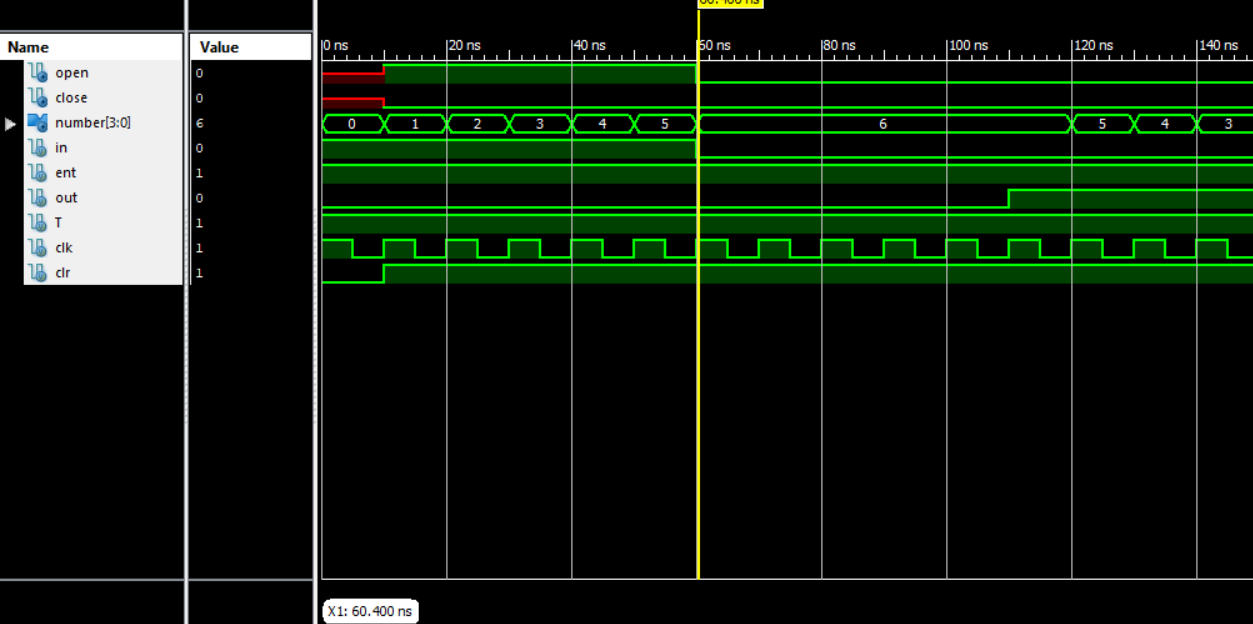
\includegraphics[width=0.8\linewidth]{s1}
\end{figure}
\begin{figure}[H]
 \centering
  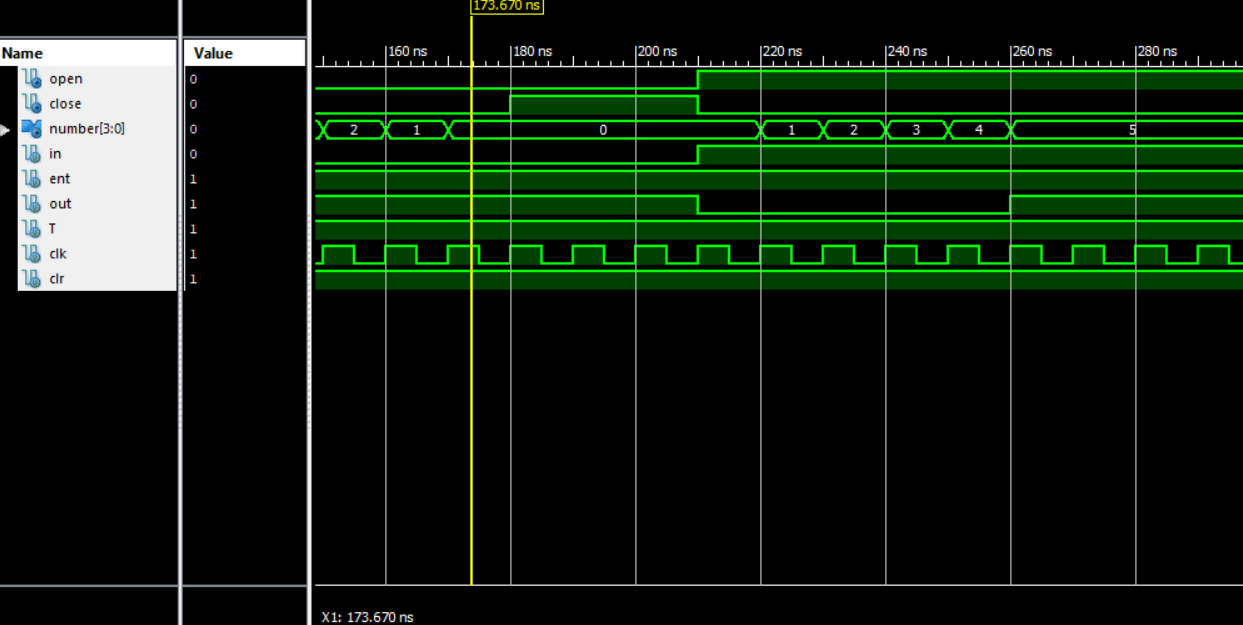
\includegraphics[width=0.8\linewidth]{s2}
\end{figure}
\begin{figure}[H]
 \centering
  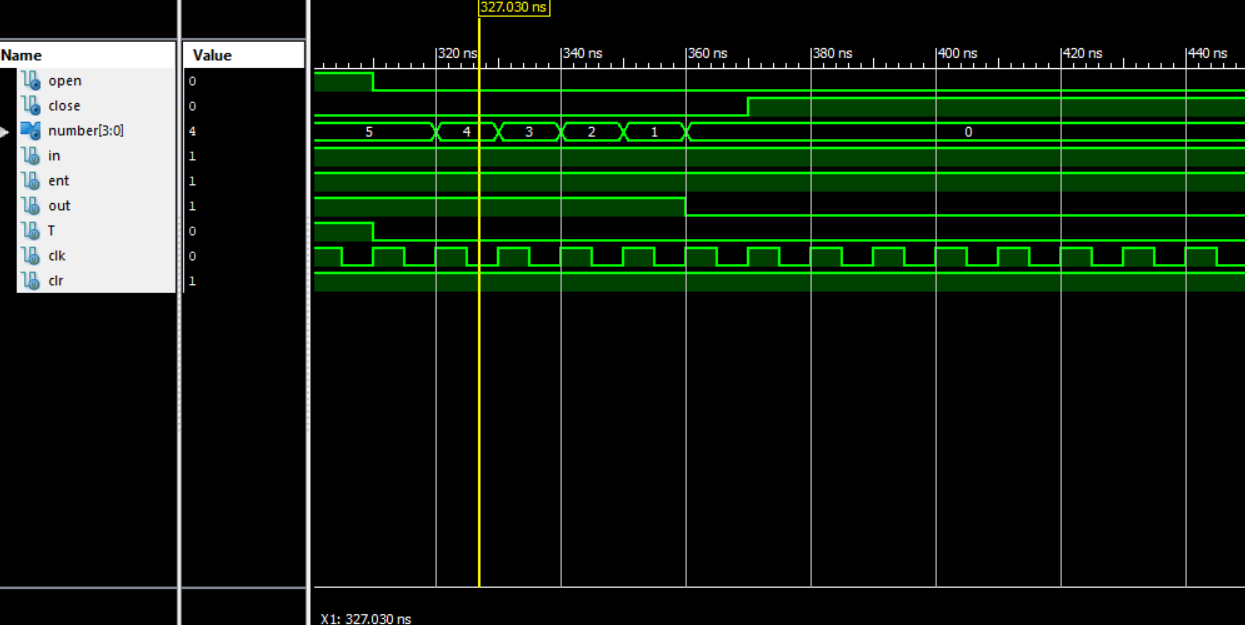
\includegraphics[width=0.8\linewidth]{s3}
\end{figure}
\end{document}